\section{Implémentation}

\subsection{Vue d'ensemble}
\begin{figure}[h]
	\centering
	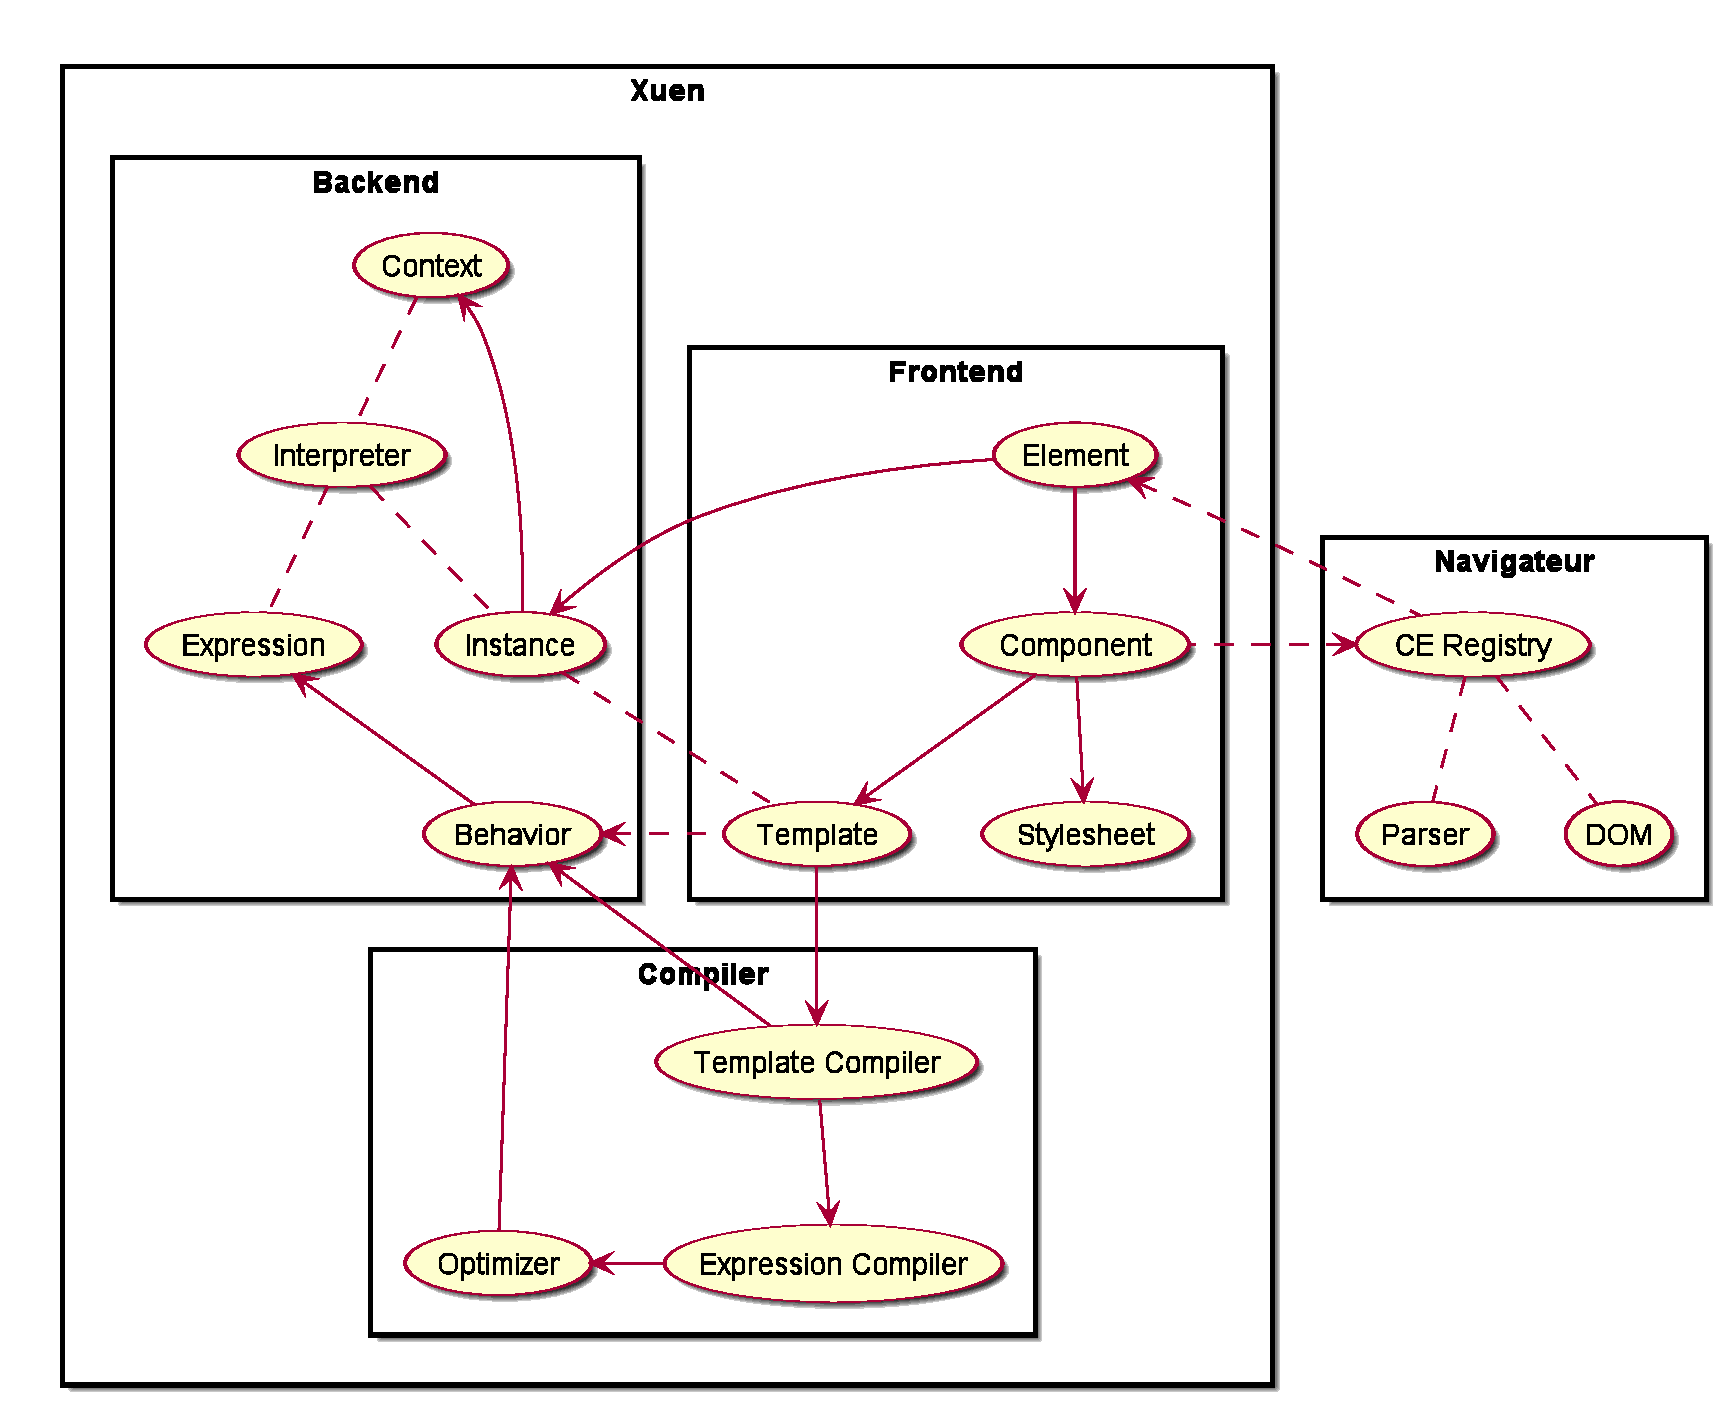
\includegraphics[width=\textwidth]{img/web_overview.eps}
	\caption{Vue d'ensemble de l'implémentation du framework Web}
	\label{fig:web-overview}
\end{figure}

\textit{Pour l'instant la spécification et l'implémentation prévue des éléments du framework web sont tous deux mentionnés dans la partie Spécifications (§~\ref{sec:web-specs}).}

\newpage
\section{Difficultés rencontrées}
\subsection{Ordre de construction des \emph{custom elements}}

\textit{Cette section nécessite rédaction}

Pour résumer le problème: les éléments customs ne sont "upgradé" (le browser invoque le constructeur de la classe associée) que lorsqu'ils sont "connectés" (leur parent de niveau racine est un Document) SAUF s'il s'agit de l'élément parent étant instancié.

Le problème est que le callback \emph{connectedCallback} est invoqué sur l'élément parent avant que les éléments enfants ne soit considérés comme connectés et upgradés. Ainsi, lorsque le template de l'élément parent est activé avec la connexion au document, les éléments enfants n'ont même pas eu l'occasion de s'initialiser et les mécanismes de data-binding explosent.

La solution adoptée est de "monter" le template de l'élément premièrement dans un sous-enfant bidon du <body>, avant de le remonter correctement dans le sous-arbre DOM de l'élément. Ce passage rapide dans le body du document déclanche l'upgrade immédiat des éléments enfants, mais ajoute son lot de nouvelle complexités. L'élément enfant est en effet considéré comme "connecté" puis "déconnecté" au cours de l'initialisation de son parent, ce qui active le template de l'élément enfant avant que l'élément parent ait eu l'occasion de s'initialiser entièrement!! Afin de prévenir ce comportement, une variable globale \texttt{forcedUpgrade} est maintenue pour déterminer si la connexion d'un élément est lié à l'upgrade forcé ou non. Dans le cas où l'élément est connecté dans le but de l'upgrader, ses callbacks \texttt{connected} et \texttt{disconnected} sont ignorés.

Jusqu'à présent, cette solution semble fonctionner dans tous les cas. Ci-dessous l'ordre des opérations observées, avec le code de construction correspondant.

\begin{lstlisting}
class Foo extends Element(Foo)
object Foo extends Component[Foo](
	"x-foo", template = html"<x-bar><x-baz></x-baz></x-bar>",
	dependencies = List(Bar, Baz))

class Bar extends Element(Bar)
object Bar extends Component[Bar](
	"x-bar", template = html"<slot></slot>")

class Baz extends Element(Baz)
object Baz extends Component[Baz]("x-baz", template = html"Baz")
\end{lstlisting}

\subsubsection{Constructeur}
\begin{lstlisting}
val foo = new Foo
println("--")
dom.document.body.appendChild(foo)
\end{lstlisting}

\begin{lstlisting}
[x-foo] Upgrade start
[x-foo] Upgrade end
--
[x-foo] Connected
[x-bar] Upgrade start
[x-bar] Upgrade end
[x-bar] Connected
[x-baz] Upgrade start
[x-baz] Upgrade end
[x-baz] Connected
\end{lstlisting}

\subsubsection{Parser HTML (connecté)}
\begin{lstlisting}
dom.document.body.innerHTML = "<x-foo></x-foo>"
\end{lstlisting}

\begin{lstlisting}
[x-foo] Upgrade start
[x-bar] Upgrade start
[x-bar] Upgrade end
[x-bar] Connected
[x-baz] Upgrade start
[x-baz] Upgrade end
[x-baz] Connected
[x-foo] Upgrade end
[x-foo] Connected
\end{lstlisting}


\subsubsection{Parser HTML (déconnecté)}
\begin{lstlisting}
val div = dom.document.createElement("div")
div.innerHTML = "<x-foo></x-foo>"
\end{lstlisting}

\begin{lstlisting}
[x-foo] Upgrade start
[x-foo] Upgrade end
\end{lstlisting}